\chapter{The SOSAA Trajectories Dataset} \label{txt:sosaa-data-chapter}

The SOSAA model is a chemistry transport model that has been actively developed in the Multi-Scale Modelling Group at the University of Helsinki since 2011 \cite{sosa-description-2011}. SOSAA was initially developed to run in stationary mode, in which it simulates the atmospheric processes near a measurement station. However, recent developments have focused on implementing a Lagrangian trajectory mode, in which emissions are picked up along the current mean meteorological trajectory that arrives at the station several days later. Please refer back to \Cref{txt:sosaa-model} for more detail on the SOSAA model and its components.

This project explores the feasibility of training a prudent Response Surface Model on SOSAA model runs using the Icarus architecture (see \Cref{txt:icarus-rsm}). We focus on the data from trajectory simulations since they provide SOSAA with external input about the emissions and meteorological conditions at every time step.

\newpar This chapter introduces the SOSAA trajectories dataset, which is published on \href{https://github.com/juntyr/sosaa-trajectories-dataset}{GitHub}. All runs in this dataset were performed with \href{https://version.helsinki.fi/putian.zhou/sosaa/-/tree/10618aa98c7470546308adf132afb0bc0735b4eb}{SOSAA@10618aa}. First, \Cref{txt:data-layout-variables} summarises the layout and variables of the dataset. Next, \Cref{txt:six-trajectories} explores the six trajectories that are included. Following on, \Cref{txt:space-time-expansion} introduces the space-time expansion procedure that is applied to all input variables, while \Cref{txt:ccn-target} details how the CCN concentration, which is used as a target variable in our experiments, is extracted from the data. Finally, \Cref{txt:feature-importance} analyses which features are most important to two simple machine learning prediction models.

\section{Description of the Dataset Layout and Variables} \label{txt:data-layout-variables}

The dataset is split into an extensive folder structure that contains the SOSAA configuration files (see \Cref{app:sosaa-settings} for an example) and the input and output NetCDF files \cite{netcdf-1989} for each of the trajectories. Each trajectory is identified by the time at which it arrives at the SMEAR II measurement station at Hyyti\"al\"a, Finland \cite{smear-station-2013}. Both the top-level \texttt{inputs/} and \texttt{outputs/} folders are split into \texttt{baseline/} and \texttt{perturbation/} directories. The former contains the baseline SOSAA runs that are used in this chapter. The \texttt{perturbation/} directory is further split by perturbation group and kind, which are explained in \Cref{txt:perturbation-generalisation}. These input directories are then split into \texttt{HYDE\_BASE\_Y2018/OUTPUT\_bwd\_\textcolor{purple}{YYYYMMDD}} folders based on the arrival date of the trajectories. Each of these folders contains an \texttt{EMISSIONS\_0422/} and a \texttt{METEO/} directory. For example, a trajectory that arrives on \textcolor{purple}{21.05.2018} at \textcolor{purple}{14:00 UTC} has the following four input files:
\begin{enumerate}
    \item aerosol emissions input: \texttt{EMISSIONS\_0422/\textcolor{purple}{20180521}\_7daybwd\_Hyde\_traj\_\textcolor{purple}{AER}\_\textcolor{purple}{10}\_L3.nc}
    \item anthropogenic emissions input: \texttt{EMISSIONS\_0422/\textcolor{purple}{20180521}\_7daybwd\_Hyde\_traj\_\textcolor{purple}{ANT}\_\textcolor{purple}{10}\_L3.nc}
    \item biogenic emissions input: \texttt{EMISSIONS\_0422/\textcolor{purple}{20180521}\_7daybwd\_Hyde\_traj\_\textcolor{purple}{BIO}\_\textcolor{purple}{10}\_L3.nc}
    \item meteorological conditions input: \texttt{METEO/METEO\_\textcolor{purple}{20180521}\_R\textcolor{purple}{10}.nc}
\end{enumerate}
Note that instead of the arrival hour \textcolor{purple}{14}, the input file names use the number of hours until midnight, \textcolor{purple}{10} in this case. In contrast to the input directories, the output folders are directly split by the full arrival time and use the natural time format instead:
\begin{enumerate}
    \setcounter{enumi}{5}
    \item SOSAA output: \texttt{\textcolor{purple}{20180521}\_T\textcolor{purple}{14}/output.nc}
\end{enumerate}
Each input and output file stores variables that are indexed by time first and often by height layer second. Since SOSAA can use arbitrary time and height resolution, these variables are linearly interpolated, which we mirror when loading these files. Biogenic emissions are a special case since they are only distributed amongst the layers reaching up to ten metres above the ground. Note that not all input variables are actually read in by the SOSAA model. For instance, only the air temperature \texttt{t}, specific humidity \texttt{q}, surface net solar radiation \texttt{ssr}, land-sea mask \texttt{lsm}, and atmospheric boundary layer height \texttt{blh} are used from amongst the meteorological variables. Thus, a model should also not be trained on them. We further exclude the layer pressure \texttt{lp} since it encourages easy overfitting on the layer height. Please refer to \Cref{app:sosaa-variables} for a complete list of the used input variables, and to \Cref{txt:ccn-target} for an explanation of how the CCN target variable is extracted from the output files. Note that both the inputs and outputs are standardised (see \Cref{txt:data-preprocessing}) based on their training data set before being used in any model.

\section{Six Representative Trajectories} \label{txt:six-trajectories}

At the start of this research project, access was provided to the inputs and outputs of 480 SOSAA trajectory runs. These 480 trajectories cover the time period from 09.05.2018 at 00:00 UTC until 28.05.2018 at 23:00 UTC, with one trajectory arriving at every full hour. In order to streamline the development and analysis of the Icarus-RSM for these trajectory datasets, we chose to focus on six example trajectories that cover different scenarios. The baseline and perturbation runs of these six trajectories and their temporal neighbours were then performed on the CSC Puhti supercomputer. The dataset of these six trajectories forms the baseline for all evaluations in \Cref{txt:icarus-evaluation-chapter} since they provide a quick overview of how a machine-learning model generalises beyond its training data across time and to unseen input scenarios.

\Cref{fig:six-trajectories-maps} shows the paths that each of the six trajectories takes over the $\geq 5$ days before it arrives at Hyyti\"al\"a. While SOSAA simulates $\geq 7$ days of the trajectory, the initial 48-hour warm-up period is excluded from the analysis. The main trajectory has a black outline and is coloured from white at the start over blue and purple to red at the time of arrival in Hyyti\"al\"a. In addition to this main trajectory, six temporally adjacent trajectories are plotted with thinner lines. Specifically, for a trajectory at time $t$, the trajectories at times $t-4\text{h}$, $t-2\text{h}$, $t-1\text{h}$, $t+1\text{h}$, $t+2\text{h}$, and $t+4\text{h}$ are plotted in blue, purple, orange, and yellow. All temporally adjacent paths should roughly line if the meteorological conditions are stable. In contrast, the trajectory that arrived in Hyyti\"al\"a on 23.05.2018 at 13:00 UTC rapidly evolved over the next four hours.

\newpar \Cref{app:six-trajectories} visually explores the input variables passed to the SOSAA model, including aerosol, anthropogenic and biogenic emissions and meteorological conditions. These inputs are summarised here alongside a description of the path that each of the six trajectories takes:
\begin{enumerate}
    \item The first trajectory starts in Sweden and travels clockwise over Russia and the Gulf of Finland before arriving in Hyyti\"al\"a on \textbf{14.05.2018} at \textbf{10:00} UTC. In this trajectory, most aerosol and anthropogenic emissions come from the time over Russia right before entering the Baltic Sea. Moreover, the temperature gradually increases until the arrival (see \Cref{fig:trajectory-inputs-14-05}).
    \item The second trajectory starts in Russia and travels counter-clockwise over the Baltics, then across to Sweden, and finally across the Gulf of Bothnia to Finland, where it arrives on \textbf{15.05.2018} at \textbf{19:00} UTC. Again, most aerosol and anthropogenic emissions originate in Russia and the Baltics (see \Cref{fig:trajectory-inputs-15-05}). While the temperature increase is less evident than the day before, the highest temperatures of up to $25 \degree \text{C}$ are limited to the final passage over Finland.
    \item The third trajectory starts in Estonia and travels clockwise across the Gulf of Finland to the west of Finland before turning towards Russia, from where it heads to its arrival at Hyyti\"al\"a on \textbf{17.05.2018} at \textbf{00:00} UTC. In this trajectory, most aerosol emissions come from the Baltics and eastern Finland (see \Cref{fig:trajectory-inputs-17-05}). Again, there is no clear temperature gradient.
    \item The fourth trajectory originates in eastern Canada, from where it crosses the Atlantic, over the southern coast of Iceland, before arriving in Norway, from where its path leads north-eastwards across Sweden and the Gulf of Bothnia to Finland, where it arrives on \textbf{19.05.2018} at \textbf{04:00} UTC. In this trajectory, most biogenic emissions come from the passage through the Nordic countries and, to a lesser extent, from Canada, with similar patterns for aerosol and anthropogenic emissions. While there is no clear pattern for the sub-zero-degree temperatures, there is a noticeable increase in above-freezing air temperatures towards the end of the trajectory (see \Cref{fig:trajectory-inputs-19-05}).
    \item The fifth trajectory starts north of Scotland, from where it travels eastwards to Norway. From Norway, it follows a clockwise bow-shape over southern Sweden and Denmark, before travelling north-eastwards towards Hyyti\"al\"a, where it arrives on \textbf{21.05.2018} at \textbf{15:00} UTC. All emissions are increased during this trajectory, with most aerosol and anthropogenic emissions occurring over Sweden. $\text{SO}_2$ emissions stand out as they are highest over Denmark and southern Norway (see \Cref{fig:trajectory-inputs-21-05}). Again, there is a clear temperature increase during the approach to Finland across the Gulf of Bothnia.
    \item The sixth and final trajectory starts north-west of Scotland from where it first travels southward over England, then sharply turns and travels northwards along the Norwegian coast before making yet another sharp turn to cross the Gulf of Bothnia from northern Sweden to southern Finland, where it arrives on \textbf{23.05.2018} at \textbf{13:00} UTC. In this trajectory, most aerosol and anthropogenic emissions originate over Scotland and England, while most biogenic emissions come from northern Sweden and Finland (see \Cref{fig:trajectory-inputs-23-05}). The sixth trajectory only shows a slight downward temperature gradient. It is worth noting that this trajectory is the least stable and rapidly transforms into an Atlantic-crossing path (similar to the 19.05. trajectory) over the next four hours.
\end{enumerate}

\begin{figure}[H]
    \centering
    \begin{subfigure}
        \centering
        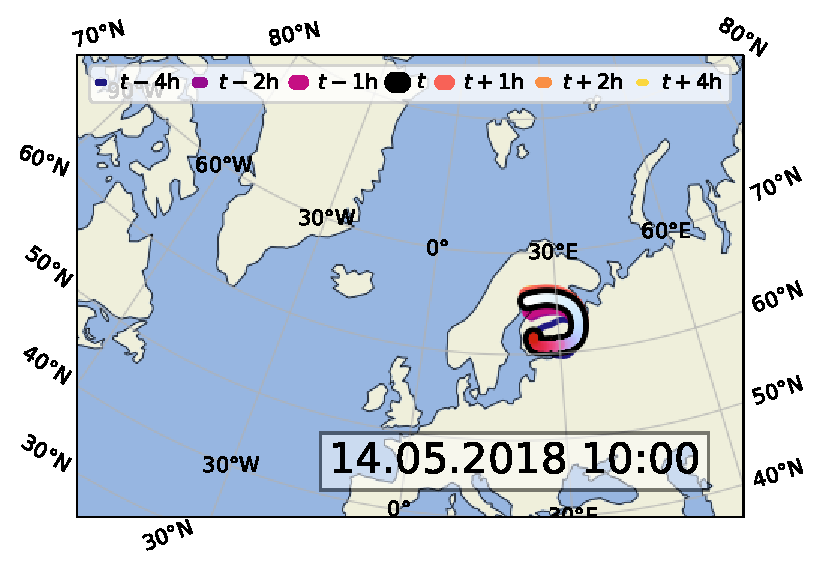
\includegraphics[width=0.49\textwidth]{sosaa-data/figures/trajectories/trajectory-14.05.2018:10.00.pdf}
    \end{subfigure}
    \begin{subfigure}
        \centering
        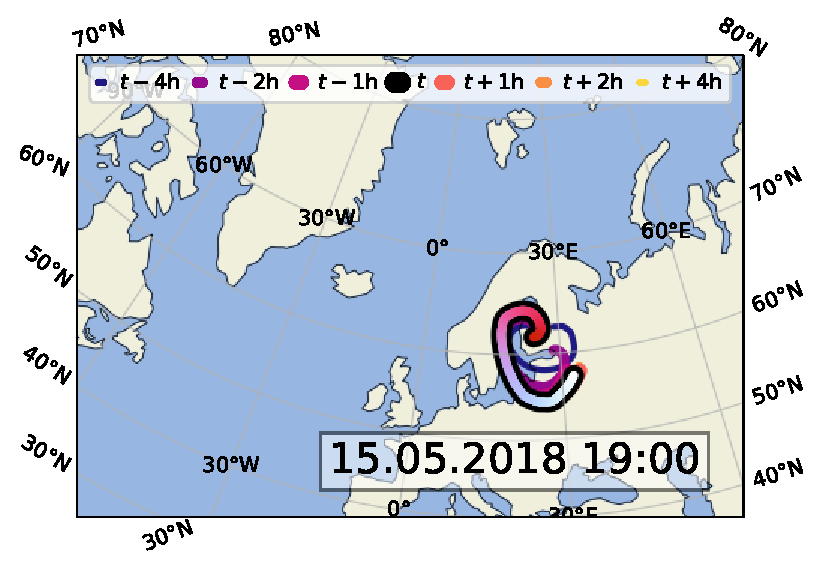
\includegraphics[width=0.49\textwidth]{sosaa-data/figures/trajectories/trajectory-15.05.2018:19.00.pdf}
    \end{subfigure}

    \begin{subfigure}
        \centering
        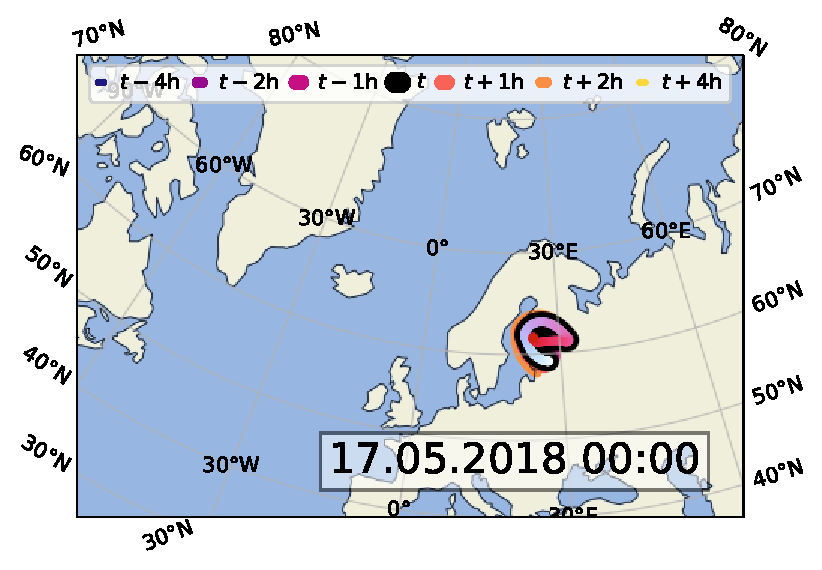
\includegraphics[width=0.49\textwidth]{sosaa-data/figures/trajectories/trajectory-17.05.2018:00.00.pdf}
    \end{subfigure}
    \begin{subfigure}
        \centering
        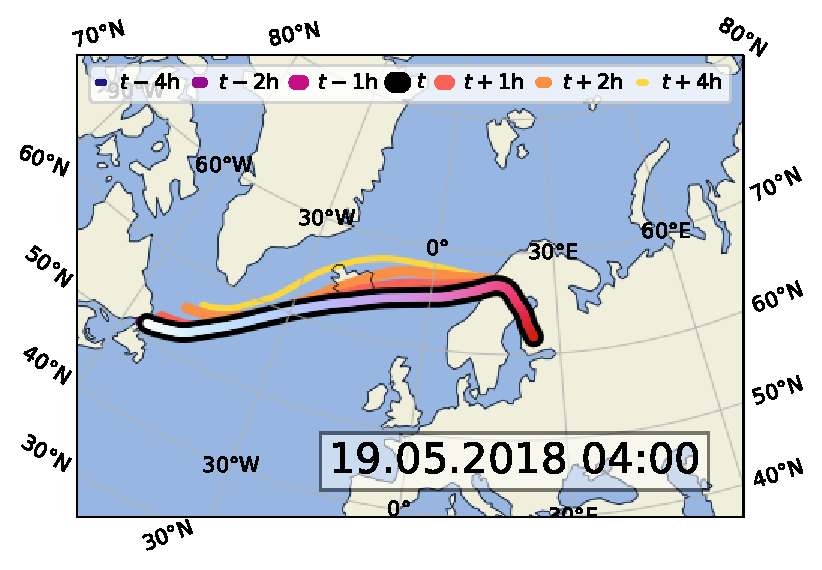
\includegraphics[width=0.49\textwidth]{sosaa-data/figures/trajectories/trajectory-19.05.2018:04.00.pdf}
    \end{subfigure}

    \begin{subfigure}
        \centering
        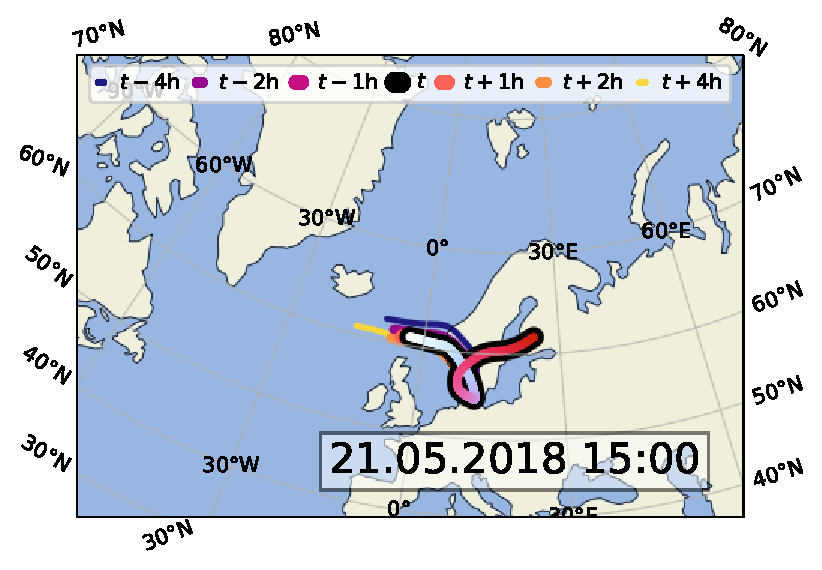
\includegraphics[width=0.49\textwidth]{sosaa-data/figures/trajectories/trajectory-21.05.2018:15.00.pdf}
    \end{subfigure}
    \begin{subfigure}
        \centering
        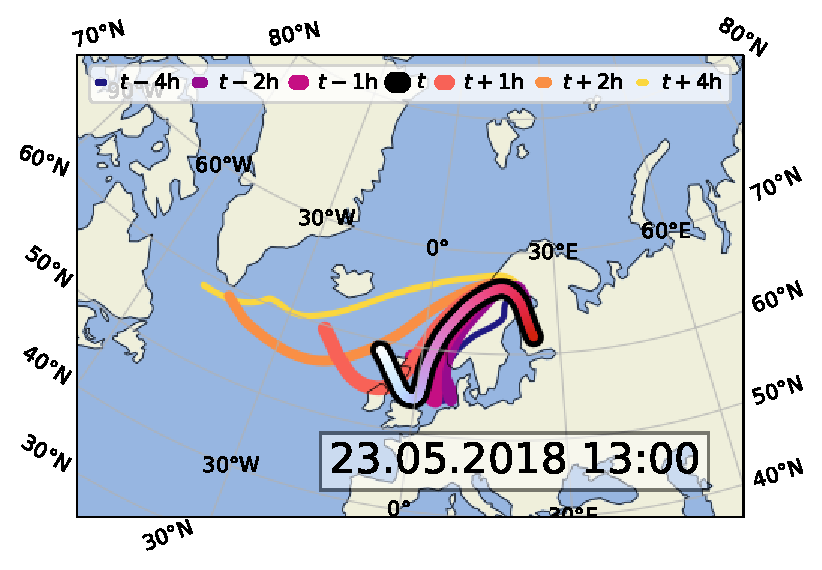
\includegraphics[width=0.49\textwidth]{sosaa-data/figures/trajectories/trajectory-23.05.2018:13.00.pdf}
    \end{subfigure}

    \caption[Maps for the six example trajectories]{Maps for the six example trajectories. Each map shows the time-coloured (see \Cref{fig:six-trajectories-ccn}) path of the trajectory that arrives at the listed time in Hyyti\"al\"a, as well as the paths of the prior and next trajectories.}
    \label{fig:six-trajectories-maps}
\end{figure}

\section{The Space-Time Expansion of Input Variables} \label{txt:space-time-expansion}

\begin{multicols}{2}
    \noindent When the SOSAA model runs in trajectory mode, it receives the current meteorological condition and emission input for every time step. In addition to these external inputs, SOSAA also carries over the internal state of every box from the previous time step. This internal state contains over two million variables across all height boxes. How can we train a Response Surface Model that independently predicts the CCN concentration for each box but also learns about the cross-box interactions? One idea is to train the RSM on the combination of the SOSAA inputs and the internal states of the previous time step. This method has the exciting extension of predicting not just the next CCN concentration but the entire state vector, allowing the emulation of the entire SOSAA model simply by stacking RSMs and running them across several time steps. While this approach would intuitively support long-term non-linear effects and produce exploding prediction uncertainty for multi-time step predictions, it would also complicate sensitivity analysis. If the CCN concentration is most sensitive to some variables of the prior state, the sensitivity would need to be evaluated recursively over several time steps and across several boxes to trace them back to the emissions. Instead, in this project, the Icarus-RSM is only trained on SOSAA's external inputs.

    \newpar How can long-term non-linear effects be captured if the RSM only receives the external inputs but cannot keep any state across time steps?

    \begin{figure}[H]
        \centering
        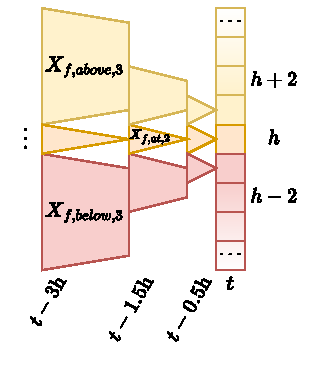
\includegraphics[width=0.49\textwidth]{sosaa-data/figures/space-time-expansion.pdf}
        \vspace{-3em}
        \caption[Input Feature Space-Time-Expansion]{Overview of the simultaneous space-time expansion of each feature $X_f(t, h)$ into $X_{f,s,i}(t, h)$. With seven time groups and an $above$, $at$, and $below$-height group, each feature is thus expanded into 21 space-time groups that summarise the influences from neighbouring SOSAA boxes.}
        \label{fig:space-time-expansion}
    \end{figure}
\end{multicols}

\noindent If the model receives the inputs not just from the current timestep and height level but from a larger range of prior time steps and surrounding boxes, it should again be able to capture these long-term effects. Therefore, we propose the following space-time expansion of the SOSAA input feature vector for the Icarus-RSM:

\begin{enumerate}
    \item \textbf{Time Expansion:} Each input feature $X_f(t)$ at time $t$ is expanded into the following seven temporally-averaged features:
    \begin{equation*}
        X_{f,i}(t) = \text{E}[\{ X_{f}(t') \given t + \Delta t_{lower, i} \leq t' \leq t + \Delta t_{upper, i} \}]
    \end{equation*}
    where $i \in 1..7$, $t_{lower} = \{ -0.5\text{h}, -1.5\text{h}, -3\text{h}, -6\text{h}, -12\text{h}, -24\text{h}, -48\text{h} \}$ and $t_{upper} = \{ -0.5\text{h}, -1\text{h}, -2\text{h},$ $-3.5\text{h}, -6.5\text{h}, -12.5\text{h}, -24.5\text{h} \}$. Note that SOSAA was configured to output predictions every $30 \text{min}$ for the trajectories dataset, which explains the half-hour time intervals.

    \item \textbf{Space Expansion:} Each input feature $X_f(h)$, where $h$ is the box height layer index, is also expanded three times into $below$, $at$, and $above$ sections which cover an expanding range of height-adjacent boxes:
    \begin{equation*}
        X_{f,s,i}(h) = \text{E}[\{ X_{f}(h') \given h + \Delta h_{s, lower, i} \leq h' \leq h + \Delta h_{s, upper, i} \}]
    \end{equation*}
    where $i \in 1..7$, $s \in \{ below, at, above \}$, and
    \begin{enumerate}
        \item $h_{at, lower} = \{ 0, 0, 0, -1, -1, -2, -2 \}$ and $h_{at, upper} = -h_{at, lower}$
        \item $h_{above, lower} = \{ 1, 1, 1, 2, 2, 3, 3 \}$ and $h_{above, upper} = \{ 1, 2, 4, 8, 16, 32, 64 \}$
        \item $h_{below, lower} = -h_{above, upper}$ and $h_{below, upper} = -h_{above, lower}$
    \end{enumerate}

    \item Note that out-of-bounds accesses for time- or space-expansion are excluded from the averaging. The $48 \text{h}$ warm-up period avoids such out-of-bounds accesses in the time expansion. However, if no data points can be averaged, e.g. when calculating $X_{f, below, i}(h)$ on the lowest layer, the result is set to zero.

    \item \textbf{Space-Time Expansion:} Both time-expansion and space-expansion are combined such that the covered space-time-area expands in both time and space simultaneously, as shown in \Cref{fig:space-time-expansion}:
    \begin{equation*}
        X_{f,s,i}(t, h) = \text{E}[\{ X_{f}(t', h') \given t + \Delta t_{lower, i} \leq t' \leq t + \Delta t_{upper, i} \wedge h + \Delta h_{s, lower, i} \leq h' \leq h + \Delta h_{s, upper, i} \}]
    \end{equation*}
\end{enumerate}

% Note: Implementation and optimisation are excluded here since they do not seem to provide value except for excess detail that then needs to be explained

\section{The CCN Target Variable} \label{txt:ccn-target}

Cloud Concentration Nuclei (CCN), which belong to aerosols in the Aitken and accumulation modes, are needed for cloud droplets and clouds to form. As \Cref{txt:aerosols} has outlined, CCN thus have a significant impact on our climate. In this project, we use the CCN concentration as the target variable. While it is usually calculated with a costly SOSAA simulation, we want to train the Icarus-RSM to predict the CCN concentration more efficiently.

\begin{figure}[H]
    \centering
    \begin{subfigure}
        \centering
        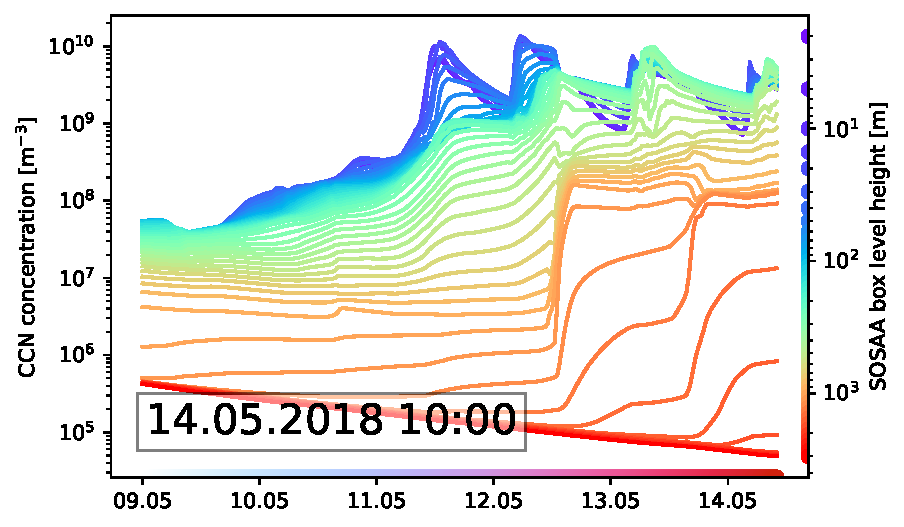
\includegraphics[width=0.49\textwidth]{sosaa-data/figures/trajectories/trajectory-14.05.2018:10.00-ccn.pdf}
    \end{subfigure}
    \begin{subfigure}
        \centering
        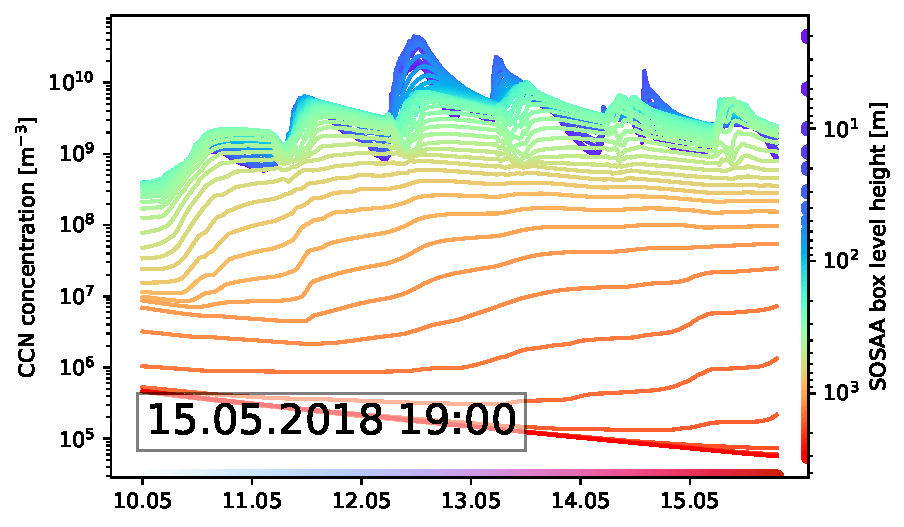
\includegraphics[width=0.49\textwidth]{sosaa-data/figures/trajectories/trajectory-15.05.2018:19.00-ccn.pdf}
    \end{subfigure}

    \begin{subfigure}
        \centering
        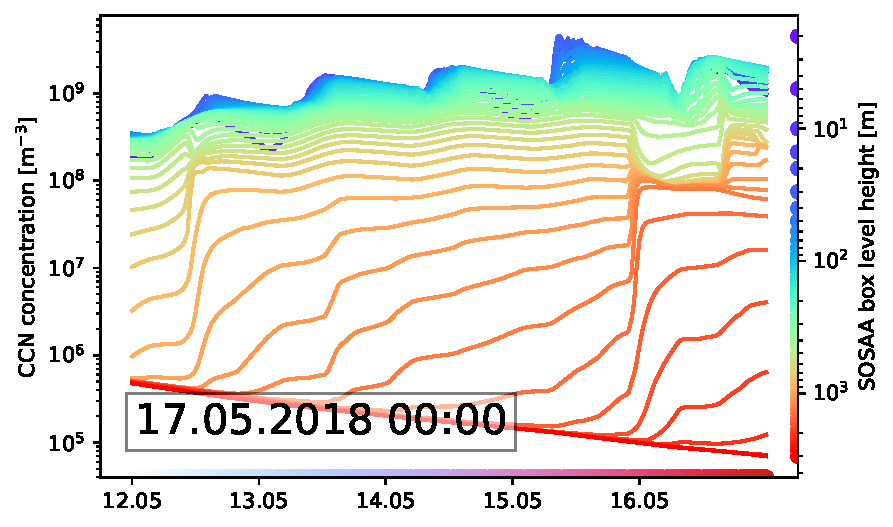
\includegraphics[width=0.49\textwidth]{sosaa-data/figures/trajectories/trajectory-17.05.2018:00.00-ccn.pdf}
    \end{subfigure}
    \begin{subfigure}
        \centering
        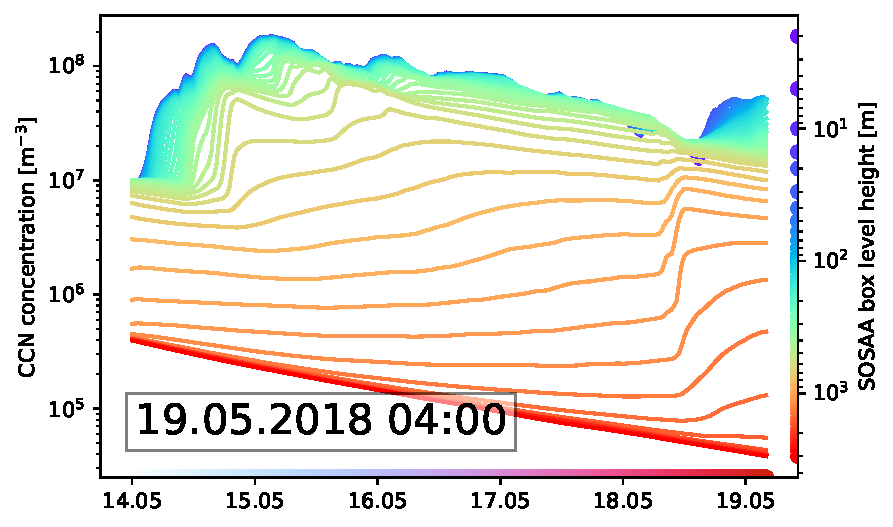
\includegraphics[width=0.49\textwidth]{sosaa-data/figures/trajectories/trajectory-19.05.2018:04.00-ccn.pdf}
    \end{subfigure}

    \begin{subfigure}
        \centering
        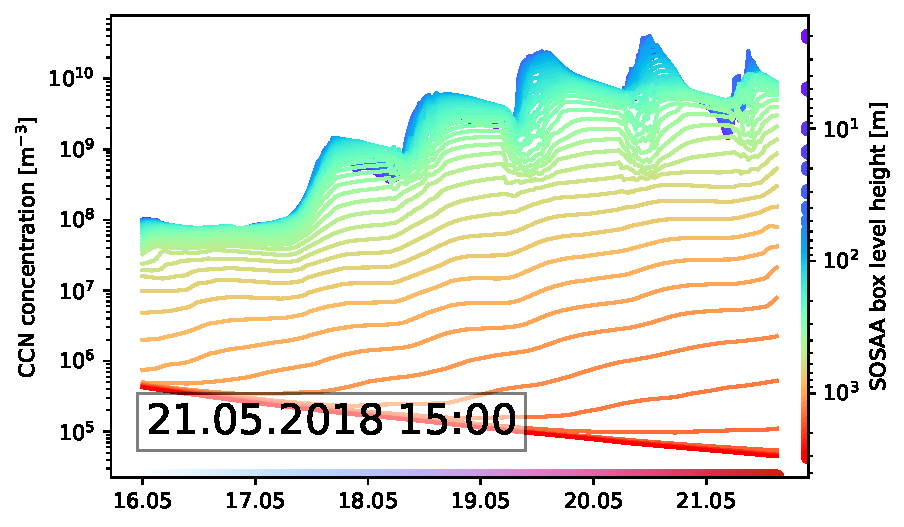
\includegraphics[width=0.49\textwidth]{sosaa-data/figures/trajectories/trajectory-21.05.2018:15.00-ccn.pdf}
    \end{subfigure}
    \begin{subfigure}
        \centering
        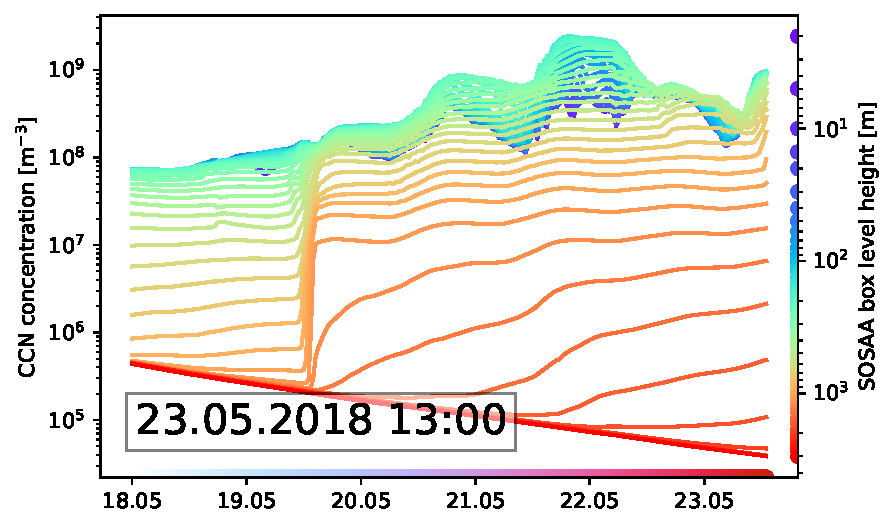
\includegraphics[width=0.49\textwidth]{sosaa-data/figures/trajectories/trajectory-23.05.2018:13.00-ccn.pdf}
    \end{subfigure}

    \caption[CCN concentration of the six example trajectories]{Per-trajectory CCN concentration over time at each of the simulated height levels. The x-axis repeats the timeline colour-coding from \Cref{fig:six-trajectories-maps}. The right y-axis shows the colour-coded height of each box level. Even though the first $48\text{h}$ are excluded for warm-up, the highest layers are still initialisation-dominated.}
    \label{fig:six-trajectories-ccn}
\end{figure}

\noindent The SOSAA simulation produces an output NetCDF file \cite{netcdf-1989} for every trajectory (see \Cref{txt:data-layout-variables}), from which we use the \texttt{dp\_dry\_fs} and \texttt{nconc\_par} variables. \texttt{dp\_dry\_fs} stores the diameter of every aerosol size-bin that SOSAA simulates. \texttt{nconc\_par} contains the number concentration for each size-bin stored for every SOSAA box height level and output time step. We count all size bins with a diameter above $80 \text{nm}$ \cite{ccn-size-2006} towards a rough estimate of the CCN concentration. \Cref{exe:ccn-concentration} below gives a sketch of the Python code to extract the CCN concentration. \Cref{fig:six-trajectories-ccn} shows the resulting CCN concentration profiles for each of the six trajectories. The height levels are spread roughly logarithmically in order to have a higher simulation resolution near the ground. Note that even though the first $48 \text{h}$ of every trajectory are used for warm-up and excluded from analysis, the highest-most layers still show after-effects from their initialisation.

\begin{listing}[H]
    \capstart % manually apply hypcap
    \begin{minted}[linenos,escapeinside=@@]{python}
import numpy as np; import pandas as pd

# Extract the CCN concentration from a SOSAA output NetCDF dataset
def get_ccn_concentration(output):
    ccn_bin_indices, = np.nonzero(output["dp_dry_fs"][:].data > 80e-9)

    return pd.DataFrame({
        "time": np.repeat(output["time"][:].data, output["lev"].shape[0]),
        "level": np.tile(output["lev"][:].data, output["time"].shape[0]),
        "ccn": np.sum(output["nconc_par"][:].data[:,ccn_bin_indices,:], axis=1).flatten(),
    }).set_index(["time", "level"])
    \end{minted}
    \caption[CCN concentration calculation procedure]{Example Python implementation of extracting the CCN concentration from the SOSAA output NetCDF file. The returned \texttt{pandas} data frame is indexed by the time step first and the height level second. The conversion from SOSAA's time format into `seconds until arrival at Hyyti\"al\"a' is omitted here for brevity.}
    \label{exe:ccn-concentration}
\end{listing}

\section{Analysing the SOSAA Input Feature Importance} \label{txt:feature-importance}

In this last section, we explore which features (see \Cref{app:sosaa-variables}) two simple machine learning models look at to make their predictions. We limit this exploration to Random Forests (see \Cref{txt:ensembles-decision-tree-random-forest}) and Pairwise Difference Regression (see \Cref{txt:padre-rf}) given their robustness with many features and little date \citeauthor{padre-rf-2021}. All feature importance experiments are evaluated by training on the combined training data from all six trajectories (see \Cref{txt:six-trajectories}) and testing on their combined validation sets. 

\begin{table}[H]
    \centering
    \begin{tabular}{ccccc} \toprule
        \multicolumn{1}{l}{} & \multicolumn{2}{c}{\textbf{Random Forest} ($MSE = 0.0012$)} & \multicolumn{2}{c}{\textbf{PADRE-RF} ($MSE = 0.156$)} \\ \cmidrule(r){2-5}
        \multicolumn{1}{c}{\textbf{emissions}} & \multicolumn{1}{c}{$\Delta MSE$} & top two $\Delta MSE$ & \multicolumn{1}{c}{$\Delta MSE$} & top two $\Delta MSE$ \\ \midrule
        \multicolumn{1}{c}{\multirow{2}{*}{\textbf{anthropogenic}}} & \multicolumn{1}{c}{$0.295$} & $0.0258$: $\text{CO}_2$ $_{(-12\text{h}, +16\text{l})}$ & \multicolumn{1}{c}{$0.22$} & $0.0264$: $\Delta$isoprene $_{(-48\text{h},+64\text{l})}$ \\
        \multicolumn{1}{c}{} & \multicolumn{1}{c}{(\#1)} & $0.0134$: pentanes $_{(-6\text{h},-8\text{l})}$ & \multicolumn{1}{c}{(\#2)} & $0.0154$: $\Delta \text{CO}_2$ $_{(-48\text{h},+64\text{l})}$ \\
        \multicolumn{1}{c}{\multirow{2}{*}{\textbf{temperature}}} & \multicolumn{1}{c}{$0.11$} & $0.0266$: temperature $_{(-48\text{h},\pm 2\text{l})}$ & \multicolumn{1}{c}{$0.355$} & $0.0887$: $\Delta$temperature $_{(-6\text{h},+8\text{l})}$ \\
        \multicolumn{1}{c}{} & \multicolumn{1}{c}{(\#2)} & $0.0064$: temperature $_{(-12\text{h},+16\text{l})}$ & \multicolumn{1}{c}{(\#1)} & $0.0706$: $\Delta$temperature $_{(-24\text{h},+32\text{l})}$ \\
        \multicolumn{1}{c}{\multirow{2}{*}{\textbf{anthr. $\text{NO}_{x}$}}} & \multicolumn{1}{c}{$0.0643$} & $0.0588$: $\text{NO}_{x}$ $_{(-12\text{h},+16\text{l})}$ & \multicolumn{1}{c}{$0.08$} & $0.0342$: $\text{NO}_{x}$ $_{(-48\text{h},+64\text{l})}$ \\
        \multicolumn{1}{c}{} & \multicolumn{1}{c}{(\#3)} & $0.0003$: $\text{NO}_{x}$ $_{(-6\text{h},-8\text{l})}$ & \multicolumn{1}{c}{(\#3)} & $0.0041$: $\Delta\text{NO}_{x}$ $_{(-48\text{h},+64\text{l})}$ \\
        \multicolumn{1}{c}{\multirow{2}{*}{\textbf{aerosols}}} & \multicolumn{1}{c}{$0.0147$} & $0.001$: $400$-$1000\text{nm}$ $_{(-48\text{h},-64\text{l})}$ & \multicolumn{1}{c}{$0.0677$} & $0.0106$: $\Delta 50$-$70\text{nm}$ $_{(-48\text{h},+64\text{l})}$ \\
        \multicolumn{1}{c}{} & \multicolumn{1}{c}{(\#4)} & $0.0008$: $10$-$20\text{nm}$ $_{(-6\text{h},-8\text{l})}$ & \multicolumn{1}{c}{(\#4)} & $0.0017$: $\Delta 400$-$1000\text{nm}$ $_{(-48\text{h},+64\text{l})}$ \\
        \multicolumn{1}{c}{\multirow{2}{*}{\textbf{anthr. $\text{SO}_{2}$}}} & \multicolumn{1}{c}{$0.0102$} & $0.0078$: $\text{SO}_{2}$ $_{(-12\text{h},+16\text{l})}$ & \multicolumn{1}{c}{$0.0621$} & $0.0081$: $\text{SO}_{2}$ $_{(-12\text{h},+16\text{l})}$ \\
        \multicolumn{1}{c}{} & \multicolumn{1}{c}{(\#5)} & $0.0003$: $\text{SO}_{2}$ $_{(-6\text{h},-8\text{l})}$ & \multicolumn{1}{c}{(\#6)} & $0.0027$: $\Delta \text{SO}_{2}$ $_{(-48\text{h},+64\text{l})}$ \\
        \multicolumn{1}{c}{\multirow{2}{*}{\textbf{biogenic}}} & \multicolumn{1}{c}{$0.0031$} & $0.0002$: $\text{CH}_2\text{O}$ $_{(-48\text{h},\pm 2\text{l})}$ & \multicolumn{1}{c}{$0.0635$} & $0.0043$: MBO $_{(-24\text{h},-32\text{l})}$ \\
        \multicolumn{1}{c}{} & \multicolumn{1}{c}{(\#6)} & $0.0001$: aldehydes $_{(-48\text{h},-64\text{l})}$ & \multicolumn{1}{c}{(\#5)} & $0.0026$: $\Delta\text{CH}_{3}\text{CHO}$ $_{(-24\text{h},-32\text{l})}$ \\
        \multicolumn{1}{c}{\multirow{2}{*}{\textbf{monoterpenes}}} & \multicolumn{1}{c}{$0.0018$} & $0.0004$: $\alpha$-pinene $_{(-48\text{h},-64\text{l})}$ & \multicolumn{1}{c}{$0.0564$} & $0.0004$: $\alpha$-pinene $_{(-24\text{h},\pm 2\text{l})}$ \\
        \multicolumn{1}{c}{} & \multicolumn{1}{c}{(\#7)} & $0.0001$: $\beta$-pinene $_{(-48\text{h},-64\text{l})}$ & \multicolumn{1}{c}{(\#7)} & $0.0002$: $\Delta \beta$-pinene $_{(-1.5\text{h},+0\text{l})}$ \\
        \multicolumn{1}{c}{\multirow{2}{*}{\textbf{sesquiterpenes}}} & \multicolumn{1}{c}{$0.0014$} & $0.0002$: sqtrps $_{(-48\text{h},-64\text{l})}$ & \multicolumn{1}{c}{$0.0554$} & $0.0001$: $\Delta$sqtrps $_{(-6\text{h},\pm 1\text{l})}$ \\
        \multicolumn{1}{c}{} & \multicolumn{1}{c}{(\#8)} & $0.0001$: sqtrps $_{(-48\text{h},\pm 2\text{l})}$ & \multicolumn{1}{c}{(\#8)} & $0.0001$: sqtrps $_{(-48\text{h},-64\text{l})}$ \\
        \multicolumn{1}{c}{\multirow{2}{*}{\textit{\textbf{ungrouped}}}} & \multicolumn{1}{c}{\multirow{2}{*}{--}} & $0.0203$: SSR $_{(-48\text{h},\pm 2\text{l})}$ & \multicolumn{1}{c}{\multirow{2}{*}{--}} & $0.0283$: $\Delta$DMS $_{(-24\text{h},-32\text{l})}$ \\
        \multicolumn{1}{c}{} & \multicolumn{1}{c}{} & $0.0113$: $\text{CH}_4$ $_{(-6\text{h},-8\text{l})}$ & \multicolumn{1}{c}{} & $0.0154$: $\Delta q_{met}$ $_{(-6\text{h},+8\text{l})}$ \\ \bottomrule
    \end{tabular}
    \caption[Permutation Feature Importance for Random Forests and PADRE-RF]{Permutation Feature Importance for Random Forests and PADRE-RF as measured by the increase in the mean-squared error. The permutations are performed both in the perturbations groups from \Cref{txt:perturbation-generalisation} and on a per-feature basis. For each group, the top two individual features are listed as well.}
    \label{tab:permutation-feature-importance}
\end{table}

\noindent First, we evaluate the \textbf{permutation importance} of each post-space-time expansion feature by shuffling the values of one feature and recording the performance drop. Features that are integral to a trained model are expected to be associated with a higher drop in prediction performance.

\Cref{tab:permutation-feature-importance} lists the permutation importances of the perturbation groups from \Cref{txt:perturbation-generalisation} and top two most important features in each group. To save space, the space-time-expanded features from \Cref{txt:space-time-expansion} are written with just their lower time bound and outer height level bound. For instance, $\text{NO}_{x}$ $_{(-6\text{h},-8\text{l})}$ refers to the averaged $\text{NO}_{x}$ emissions that occurred between $6\text{h}$ and $3\text{h}$ before the current time step and within all height layers starting two below the current layer and expanding down up to eight layers below. Note that since SOSAA is usually run with around $50$ height layers, any features using, e.g. $+64\text{l}$ effectively include all height layers above the current one. Please refer back to \Cref{txt:space-time-expansion} for details on the space-time expansion of all features.

First, we notice that anthropogenic emissions and air temperature are the most important, followed by anthropogenic $\text{NO}_{x}$ emissions. Second, the importance order of perturbation groups is almost the same for both Random Forests and PADRE-RF, apart from anthropogenic and temperature as well as $\text{SO}_2$ and biogenics switching ranks. Note that low perturbation importance does not necessarily mean that this feature has low relevance in the real world. For instance, the lower importance of all biogenic emissions may also be related to the lower variation in these inputs across the dataset (see \Cref{fig:trajectory-inputs-14-05}, \Cref{fig:trajectory-inputs-15-05}, and \Cref{fig:trajectory-inputs-17-05}). Third, we notice that since biogenic emissions occur near the ground, features that look at a large range of height layers below have high importance. In contrast, the models assign high importance to averaging all anthropogenic emissions in height layers above the current one. Fourth, we can see that PADRE-RF has a less steep drop-off in importance, especially for biogenic, monoterpene, and sesquiterpene emissions. Thus, we hypothesise that PADRE-RF may have a higher capacity than Random Forests at predicting changes in CCN concentrations for perturbations of these groups. This hypothesis is tested in \Cref{txt:perturbation-generalisation}.

\newpar Second, we investigate the minimal set of features needed to achieve good predictive performance. In particular, we look for the smallest set of features such that adding a new feature no longer brings an improvement that exceeds a set threshold, here $\Delta MSE_{min} = -0.01$. In this sequential feature selection process, we first train one model per feature and then choose the feature with the lowest prediction error, evaluated using $k$-fold cross-validation. Next, we iterate over all remaining features and check which second feature can be selected to produce the best two-feature model. Since Random Forests can be very accurate with very few features by overfitting on noise in the data, we instead use linear regression models in this investigation. In order to still capture non-linear processes, we expand the selected features to their third-order polynomial combinations. To avoid the $\text{O}(F^3)$ complexity for $F$ features, we approximate this polynomial expansion with just $4F$ features using the Nystr\"om method \cite{nystroem-kernel-2000, nystroem-fourier-2012}, as implemented in the \texttt{scikit-learn} library \cite{scikit-learn-2011}.

\newpar Training on the standard features, sequential feature selection selects the following features with $MSE = 0.321$:
\begin{flalign*}
    \quad \{ \quad & && \\
    & \text{temperature }_{(-24\text{h},+32\text{l})}, \text{temperature }_{(-24\text{h},-32\text{l})}, \text{temperature }_{(-6\text{h},+8\text{l})}, \text{temperature }_{(-12\text{h},+16\text{l})}, && \\
    & \text{anthropogenic NH}_{3}\text{ }_{(-24\text{h},-32\text{l})}, \text{aerosols } 200\text{-}400\text{nm }_{(-24\text{h},-32\text{l})}, && \\
    \quad \} \quad & &&
\end{flalign*}
In comparison, the following pairwise difference regression features are chosen with $MSE = 0.527$:
\begin{flalign*}
    \quad \{ \quad & && \\
    & \Delta \text{temperature }_{(-24\text{h},+32\text{l})}, \text{temperature }_{(-48\text{h},+64\text{l})}, \text{temperature }_{(-24\text{h},-32\text{l})}, && \\
    & \Delta \text{biogenic isoprene }_{(-3\text{h},-4\text{l})}, \Delta \text{temperature }_{(-24\text{h},-32\text{l})}, \Delta \text{temperature }_{(-48\text{h},-64\text{l})}, && \\
    & \Delta \text{biogenic CO }_{(-3\text{h},-4\text{l})}, \Delta \text{biogenic CO }_{(-3\text{h},+4\text{l})}, && \\
    \quad \} \quad & &&
\end{flalign*}
We can see that, unlike permutation importance, sequential feature selection identifies temperature as the most important feature. In fact, the temperature features create the most significant reductions in the prediction error for both Random Forests and Pairwise Difference Regression. In contrast, the later-selected features only provide more minor improvements that do not significantly exceed the $\Delta MSE_{min} = -0.01$ threshold. One possible explanation might be that temperature is a dominant variable. In this case, temperature perturbations should have the largest impact on CCN concentrations in \Cref{txt:perturbation-generalisation}. The Icarus RSM should predict both temperature and other perturbations well, the latter simply because they would not have a significant impact. However, it is also possible that temperature simply is the only variable that has significant independent variation within the dataset. In this case, the Icarus RSM would succeed in predicting temperature perturbations but fail at predicting the change in CCN for other perturbations.
